\documentclass{standalone}
\usepackage{tikz}
\usetikzlibrary{er,positioning}
%\tikzstyle{attribute} = [circle, draw, text width=6em, text centered, minimum width=3em]
%\tikzstyle{entity} = [rectangle, draw, text width=6em, text centered, minimum width=5em, minimum height=2.5em]
%\tikzstyle{relation} = [diamond, draw, text width=6em, text centered, minimum width=6em, aspect=2]

\begin{document}



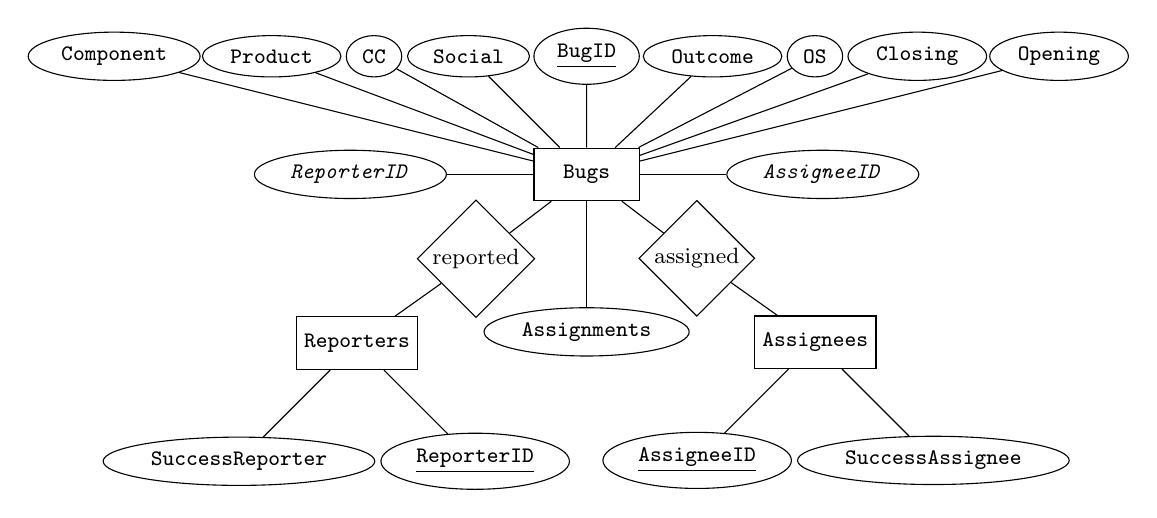
\begin{tikzpicture}[node distance=0.5cm, auto, >=stealth]
{\footnotesize
	
\node[entity] (reporters) {\texttt{Reporters}}
	[grow=down,sibling distance=3cm]
	child {node[attribute] {\texttt{SuccessReporter}}}
	child {node[attribute] {\underline{\texttt{ReporterID}}}};

\node[relationship] (reports) [above right= of reporters] {reported};

\node[entity] (bugs) [above right = of reports] {\texttt{Bugs}}
	[grow=up,sibling distance=2cm]
	child {node[attribute, ,xshift=-50mm] {\texttt{Opening}}}
	child {node[attribute,xshift=-48mm] {\texttt{Closing}}}
	child{node[attribute,xshift=-41mm] {\texttt{OS}}}
	child {node[attribute,xshift=-34mm] {\texttt{Outcome}}}
	child {node[attribute,xshift=-30mm] {\underline{\texttt{BugID}}}}
	child {node[attribute,xshift=-25mm] {\texttt{Social}}}
	child {node[attribute,xshift=-17mm] {\texttt{CC}}}
	child {node[attribute,xshift=-10mm] {\texttt{Product}}}
	child {node[attribute,xshift=-10mm] {\texttt{Component}}}
	child [grow=left,level distance=3cm]{node[attribute] {\textit{\texttt{ReporterID}}}}
	child [grow=right,level distance=3cm]{node[attribute] {\textit{\texttt{AssigneeID}}}}
	child [grow=down,level distance=2cm]{node[attribute] {\texttt{Assignments}}};

\node[relationship] (assigns) [below right= of bugs] {assigned};

\node[entity] (assignees) [below right = of assigns] {\texttt{Assignees}}
[grow=down,sibling distance=3cm]
child {node[attribute] {\underline{\texttt{AssigneeID}}}}
child {node[attribute] {\texttt{SuccessAssignee}}};

\draw (reporters)--(reports)--(bugs)--(assigns)--(assignees);				
}
\end{tikzpicture}


\end{document}